\chapter{Project in details}

\section{Architecture overview}
The system consists of multiple different applications running in a single application container (the plugin application) adapted the needs of the different user groups. Every application implements a specific group of aspect of the system. To enforce a consistent user experience and to provide only a single Windows application to the users, the system uses the plugin pattern.
\par
The different applications plugged into the plugin application are all structured according to strict layer architecture, i.e. the layer architecture is the top level structural decomposition used.	
\par
The system consists of multiple different applications running in a single application container (the plugin application) adapted the needs of the different user groups. Every application implements a specific group of aspect of the system. To enforce a consistent user experience and to provide only a single Windows application to the users, the system uses the plugin pattern.
\par
The different applications plugged into the plugin application are all structured according to strict layer architecture, i.e. the layer architecture is the top level structural decomposition used.
%
\subsection{Plugin application concept}
All applications are built as plugins running inside the plugin application. At startup, this plugin application will load all the deployed plugin assemblies. These assemblies contain entry point classes for the module: the plugin classes. Then to find those plugin classes, the plugin application searches in the plugin assemblies for the implementer. It will interact with those plugins by calling methods of this interface. The plugin application can also communicate with all the application windows to send them toolbar commands like close, refresh, etc.
\begin{figure}[ht]\centering
	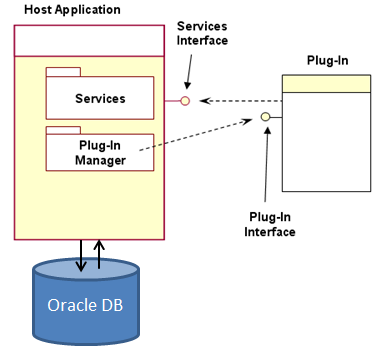
\includegraphics[width=.7\textwidth]{pic_plug_arch.png}
	\caption{Plugin architecture.}
\end{figure}
%

\section{Structural decomposition}
N-layer architecture is all about separating different types of functionality. The common logical separation is into a Presentation layer, a Business layer, and a Data layer. These may exist on a single machine or on many separate machines – the logical architecture does not define those details. A physical n-tier is quite different from logical n-layer architecture. In n-tier architecture, the application is spread across multiple machines with different functions: a client, a web server, an application server, a database server, and so on. There is a relationship between an application's logical and physical architectures: the logical architecture always has at least as many layers as the physical architecture has tires. There may be more logical layers than physical tiers (because on physical tier can contain several logical layers), but never fewer.
\par
The current application is structured into the layers as the figure \ref{fig_layers}. The layering is strict, i.e. it is not allowed to skip a layer. The only exceptions are the common technical components, which can be used by Presentation, Business and Data Access layer. Below the layer name, the diagram also shows the main frameworks/ tools used in the corresponding layer, e.g. the Data Access layer is built based on NHibernate.

\begin{figure}[ht]\centering
	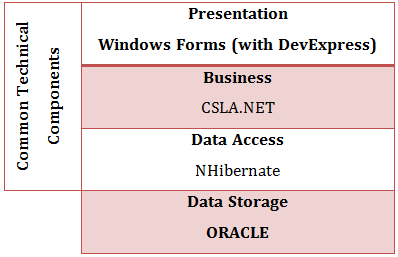
\includegraphics[width=.67\textwidth]{pic_layers.PNG}\label{fig_layers}
	\caption{Application architecture modeling overview.}
\end{figure}

\par
The logical layers are deployed as a rich client, i.e. Presentation, Business and Data Access layer are running on one machine as a single application. The database is running on a separate server, i.e. it is a 2-tier physical deployment.
\par
Having clean separation between these layers makes the application more maintainable, because changing one layer often has minimal impact on the other layers. Properly designed logical n-layer architecture provides the following benefits: 
\begin{itemize}
	\item Easier maintenance
	\item Better reuse of code
	\item Better team-development experience
	\item Higher clarity in coding
\end{itemize}

\par
On the other hand, properly chosen physical n-tier architecture can provide the following benefits:
\begin{itemize}
	\item Performance
	\item Scalability
	\item Fault tolerance
	\item Security
\end{itemize}
%

\subsection{Presentation layer}
The presentation uses Windows Forms with DevExpress controls to significantly improve productivity and provide a better user experience for consumers. DevExpress has made the application development easier by providing easy to use controls for Windows Forms. DevExpress~\cite{DED} controls use standard Visual Studio development methods. They are one of the most stable and easy to use tools that can cut down your development time up to 50\%. The CSLA framework, is used in business layer, also provides some advanced features for data binding and validation. The application uses these features to bind Windows Forms UI to the Business layer.
%

\subsection{Business layer}
The Business layer is built using a different domain model for different use cases. Business logic includes all business rules, data validation, manipulation, processing, and authorization for the application. The business logic must reside in a separate layer from the presentation code. It must implement all the business logic, because it is the only point of central control and maintainability. 
\par
CSLA .NET is the heart of Business layer that provides a standard way to create robust object oriented programs using business objects. Business objects are objects that abstract business entities in an object oriented program. A business object encapsulates all the data and behavior (business logic and rules) associated with the object it represents. For example, an OrderEdit object will contain the data and business rule implementations necessary for the application to correctly allow the user to edit order information. Business objects created using CSLA .NET fully supports data binding for all Microsoft .NET UI technologies, including Windows Forms.
%

\subsection{Data Access layer}
Data access code interacts with the Data Storage layer to retrieve, insert, update, and delete information. The Data access layer does not actually manage or store data; it merely provides an interface between the business logic and database.  By isolating the data access code into a specific layer, the impact of later changes, i.e. data access technology, is limited to a smaller part of the application.
\par
NHibernate~\cite{NRD}, an object-relational mapping (ORM) tool, is used in the data access layer to map between the object oriented business logic and the relational data in a data store. It also provides data query and retrieval facilities. It generates the SQL commands and relieves the developer from manual data set handling and object conversion, keeping the application portable to most SQL databases, with database portability delivered at the very little performance overhead.
%

\subsubsection{Concurrency management}
The system uses optimistic locking to detect concurrent modifications on the data. The strategy used is therefore “first writer wins”. The assumption behind this is that conflicts only occur rarely and user accepts to lose their work under these circumstances.
Optimistic locking is implemented by using the version column ROW\_VERSION in tables.
%

\subsubsection{Storing data}
The mapping between CSLA business object and NHibernate data object is required to store data. To update new data, rehydrating the NHibernate data access object is performed from the database first, and then maps the CSLA business object to the data access object. The data objects only persist themselves to a database if their data has been changed. Data creation, retrieval, updates, and deletes are performed by clearly defined methods of the business object associated with the data. Data access logic is clearly separated from business logic, typically using a repository pattern or other mainstream object-oriented programming techniques.
\par
The data access layer provides a repository per root object of the data object. The Repository is implemented based on NHibernate, which maps between the database and the data object.
\par
A Unit of Work bundles together all the operations on the database belonging to one business action. The unit of work creates and manages the NHibernate session. Every interaction with the database must be part of a Unit of Work.
%

\subsubsection{Data Storage layer}
All the data are stored in already existing Oracle schemas. There are many challenges when using existing schemas such as all tables do not have foreign key constraints defined, many tables do not have unique keys or composite keys is already in place. Database changes can be requested such as adding artificial key columns, adding row version columns before attempting to implement an ORM tool. 
Chances are that the lack of foreign key constraints is masking underlying issues with the integrity of the data. While NHibernate will work without every foreign key being defined with a constraint, it makes the database vulnerable to integrity violations, and it slows the database down because the Query Optimizer uses this information in its task of determining the best query strategy.
%

\subsection{Solutions in short}
During the six-month working at ELCA, I solved most of the difficulties mentioned in section \ref{sec:challenges} using my knowledge from courses in PUF as well as the colleagues' effective support.  In this section, some of our solutions proposed and applied in the project will be discussed. 
\par
To solve the data inconsistency problem, no specific solution was proposed.  There is no conflict with the previous version accepted but as mentioned above, the missing foreign key might lead to inconsistency. We currently solve this inconsistency by carefully check the data before implementing ORM tool. We also add the artificial keys to some of the tables in order to solve the composite key problem.  The last problem with the oracle database application is the uniqueness constraints. This problem must be solved by checking the data in the customers' database, in case there is any conflict, we need to wait for the official discussion between our team specs and the customers for the more specific requirements.
To improve performance, we apply the static cache and indexing for data. The performance is improved dramatically. This makes the system extensibility and scale up in the future. Besides that, I also use NHibernate Profiler regularly to detect in advance possible performance problem such as select N+1 problem. The select N+1 problem is described carefully in the website Hibernating Rhinos~\footnote{http://www.hibernatingrhinos.com/products/nhprof/learn/alert/selectnplusone}. NHibernate Profiler gives us relevant data about the number of queries, session usage, query durations and warnings of possible performance bottlenecks.
\par
The retrieved data model must be mapped to followed parent-child relationship of CSLA model. Some of the design patterns are applied to solve the problem. At the beginning, all of the documents must be strictly followed. Later, the code base is no longer matched to the requirements and new patterns as well as the code must be developed flexibly to follow all the specs.
%

